\begin{frame}
  \frametitle{Influence diagnostics for MLMs}

  \begin{itemize}
  \item Influence measures and diagnostic plots are well-developed for univariate LMs
    \begin{itemize}
    \item Influence measures: Cook's D, DFFITS, dfbetas, etc.
    \item Diagnostic plots:  Index plots, \code{car:::influencePlot()} for LMs
    \item However, these are have been unavailable for MLMs  
    \end{itemize}
  \item
    The \package{mvinfluence} now provides:
    \begin{itemize}
    \item Calculation for multivariate analogs of univariate influence measures
    (following Barrett \& Ling, 1992)
    \item Provides deletion diagnostics for subsets of size $m \ge 1$.
    \item e.g., $m=2$ can reveal cases of \alert{masking}.
    \item Extension of \code{influencePlot()} to the multivariate case.
    \item A new plot format: leverage-residual (LR) plots.
    \end{itemize}
  \end{itemize}
\end{frame}

\begin{frame}
  \frametitle{Influence diagnostics for MLMs: Example}
  For the Rohwer data:

% two figs side-by-side
  \begin{minipage}[c]{.5\textwidth}
   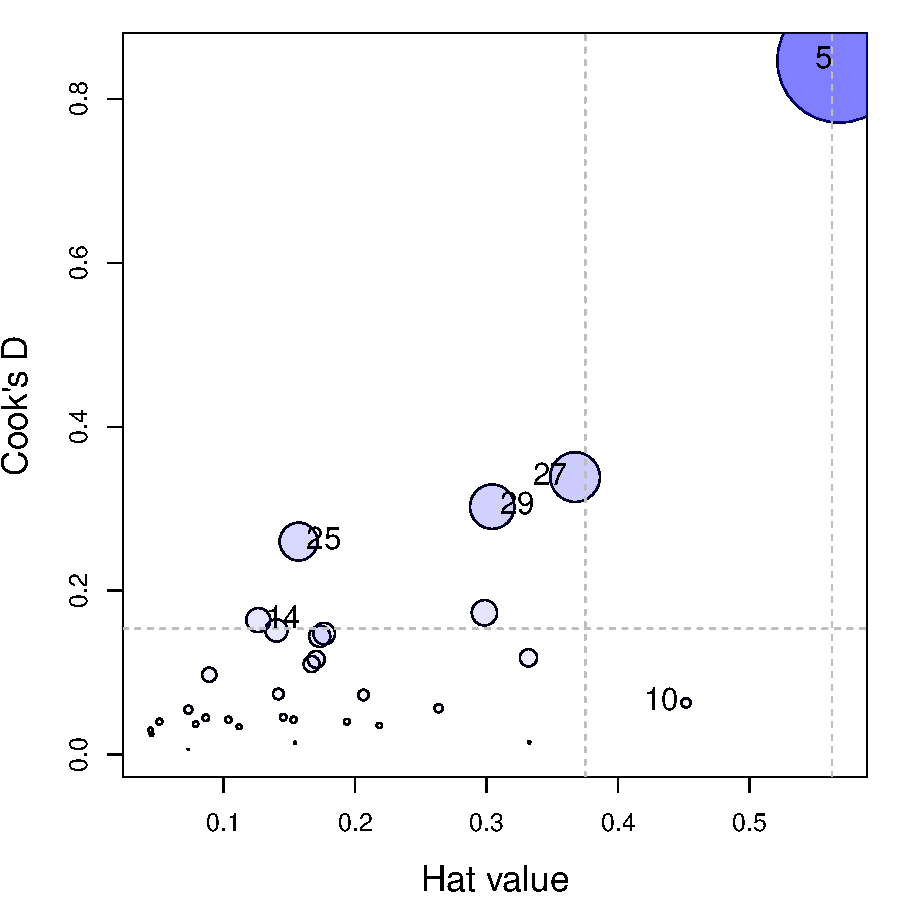
\includegraphics[width=1\linewidth,clip]{figures/rohwer-influence-cookd.pdf}
   \end{minipage}%
  \hfill
  \begin{minipage}[c]{.5\textwidth}
   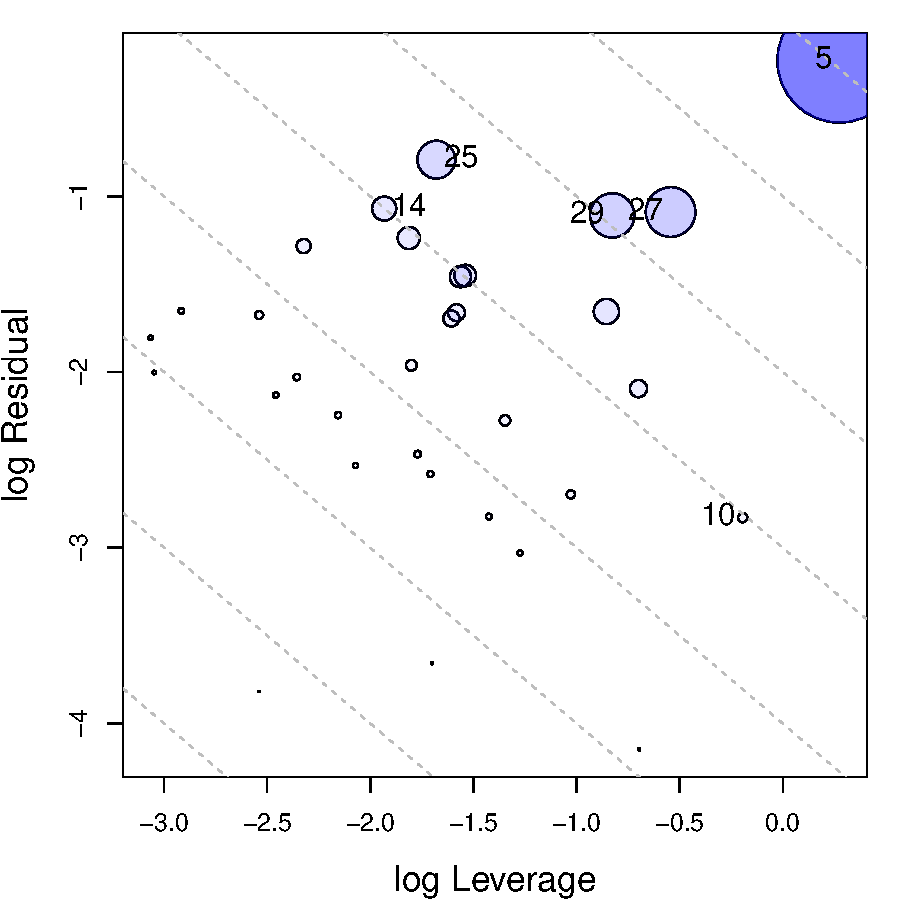
\includegraphics[width=1\linewidth,clip]{figures/rohwer-influence-LR.pdf}
  \end{minipage}

\end{frame}
